\documentclass{beamer}
%\usepackage[none]{hyphenat}
\usepackage{multicol}
\usepackage{xcolor}
\usepackage{listings}
\usepackage{minted}

\usetheme[progressbar=frametitle]{metropolis}
\setbeamertemplate{frame numbering}[fraction]
\useoutertheme{metropolis}
\useinnertheme{metropolis}
\usefonttheme{metropolis}
\usecolortheme{spruce}
\setbeamercolor{background canvas}{bg=white}

\definecolor{mygreen}{rgb}{.8,.5,.25}
\usecolortheme[named=mygreen]{structure}


%New colors defined below
\definecolor{codegreen}{rgb}{0,0.6,0}
\definecolor{codegray}{rgb}{0.5,0.5,0.5}
\definecolor{codepurple}{rgb}{0.58,0,0.82}
\definecolor{backcolour}{rgb}{0.95,0.95,0.92}
\definecolor{light-gray}{gray}{0.9}
\newcommand{\code}[1]{\colorbox{light-gray}{\texttt{#1}}}

%Code listing style named "mystyle"
\lstdefinestyle{mystyle}{
  backgroundcolor=\color{backcolour}, commentstyle=\color{codegreen},
  keywordstyle=\color{magenta},
  numberstyle=\tiny\color{codegray},
  stringstyle=\color{codepurple},
  basicstyle=\ttfamily\scriptsize,
  breakatwhitespace=false,         
  breaklines=true,                 
  captionpos=b,                    
  keepspaces=true,                 
  numbers=left,                    
  numbersep=5pt,                  
  showspaces=false,                
  showstringspaces=false,
  showtabs=false,                  
  tabsize=2
}

%"mystyle" code listing set
\lstset{style=mystyle}

\title{Continuous Integration and Development}
\subtitle{\textbf{Fastlane with Jenkins}}
\author{Iktiar Ahmed Imon}
\institute{\large \textbf{\color{red}{Kona Software Lab Ltd.}}}
\date{\today}

%\setbeamercovered{transparent=5}

\begin{document}
\metroset{block=fill}

\begin{frame}
    \titlepage
\end{frame}

\begin{frame}[t]{CI/CD} 
    \vspace{3pt}
    Continuous Integration and Development is helpful to deliver code changes more frequently and reliably.
    \vspace{3pt}

    \begin{block}{Continuous Integration}
        \vspace{0.5em}
            Continuous Integration is the practice of automating the integration (\textcolor{magenta}{test before merging code}) of code changes from multiple contributors into a single project.
    \vspace{0.5em}
    \end{block}

    \vspace{3pt}

    \begin{block}{Continuous Development}
        \vspace{0.5em}
            Continuous Delivery automatically deploys all code changes to a testing and/or production environment after the build stage.
        \vspace{0.5em}
    \end{block}

\end{frame}

\begin{frame}[t]{Fastlane}
    
\includegraphics[scale=0.25]{fastlane}\centering
    \vspace{3pt}
    \begin{itemize}
        \item Fastlane is a toolchain that uses the Xcode command line toolchain to automate a vast number of tasks.
       \item Automate your development and release process
       \item Fastlane also supports \colorbox{pink}{$Android$} projects. This makes it viable for native and cross platform development i.e. React Native, Flutter projects.
    \end{itemize}
\end{frame}



\begin{frame}[t]{Fastlane Features}
    It provides below facilities - 
    \vspace{3pt}
    \begin{enumerate}
        \item \textbf{Capture screenshots automatically}
            \begin{itemize}
                \item Automatically capture localized screenshots for each language and device your app supports.
            \end{itemize}
        \item \textbf{Distribute beta builds}
            \begin{itemize}
                \item Easily publish new beta builds to testers so you can get valuable feedback, fast.
            \end{itemize}
        \item \textbf{App store deployment}
            \begin{itemize}
                \item Automatically submit new versions of your app for review.
            \end{itemize}
        \item \textbf{Automate Code Signing}
            \begin{itemize}
                \item Store your code signing identities and profiles in your own private, encrypted git repository to securely sync them across machines.
            \end{itemize}
    \end{enumerate}
\end{frame}

\begin{frame}[fragile]{Example of Fastlane Script}
    Fastlane helps you to create scripts (using \colorbox{pink}{$ruby$}) 
    \vspace{3pt}
    \begin{lstlisting}[language=Ruby]
      lane :beta do
		    increment_build_number
		    build_app
		    upload_to_testflight
	    end \end{lstlisting}
	
	
	\begin{lstlisting}[language=Ruby]
	    lane :appstore do
		    capture_screenshots
		    build_app
		    upload_to_app_store
		    slack
	    end \end{lstlisting}
	Think a lane as a method with a set of build “steps”, where each step is represented for a Fastlane Action. And the lanes with their building steps are defined in the Fastfile file.
\end{frame}

\begin{frame}{Working With Fastlane}
    \begin{itemize}
        \item Install Fastlane first
        \item Create \colorbox{pink}{$fastlane$} folder where your $.xcodeproj$ file resides with associated files.
    \end{itemize}
    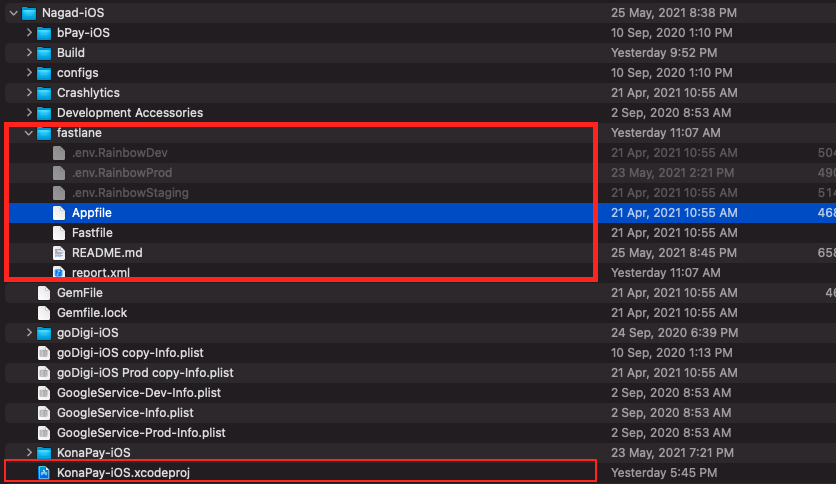
\includegraphics[scale=0.25]{fastlane_integration}\centering
    \begin{itemize}
        \item You can create $.env.AnyName$ file to run a $lane$ with different configuration. It is a mapping file.
    \end{itemize}
    
    
\end{frame}

\begin{frame}{Run a lane with terminal}
    \begin{itemize}
        \item Open your terminal at where your $.xcodeproj$ file resides.
        \item It will automatically finds all declared $lanes$.
        \item run \code{fastlane laneName --env AnyName} \textcolor{blue}{// \code{--env} is optional if you have declared any}
    \end{itemize}
    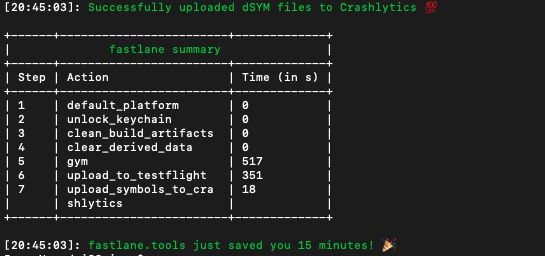
\includegraphics[scale=0.45]{fastlane_output.png}\centering
\end{frame}


\begin{frame}{Shortcomings of fastlane}
    \begin{itemize}
        \item Fastlane is not SCM(remote repository) aware.
        \item Here comes \colorbox{pink}{$Jenkins$} or other automation servers.
        \item Fastlane can be integrated effortlessly into existing popular CI services i.e. Jenkins, Bitrise, CircleCI, Travis, Azure DevOps.
    \end{itemize}
    
\includegraphics[scale=0.25]{fastlane.png}\centering
\end{frame}


\begin{frame}{Jenkins}
    
\includegraphics[scale = 0.21]{jenkins.png}\centering
    \begin{itemize}
        \item Jenkins is a free and open source automation server.
        \item It is written in java.
        \item It's a plugin based solution to automation. The Jenkins community offers 1700+ plugins that enable Jenkins to integrate with virtually any tool.
        \item It helps automate the parts of software development related to building, testing, and deploying, facilitating continuous integration and continuous delivery.
    \end{itemize}
\end{frame}

\begin{frame}{A little bit history}
    \only<1>{
        \begin{itemize}
            \item The Jenkins project was started in 2004 (originally called \textbf{\textit{Hudson}}) by \textbf{Kohsuke Kawaguchi}, while he worked for Sun Microsystems. Kohsuke was a developer at Sun and got tired of incurring the wrath of his team every time his code broke the build. He created Jenkins as a way to perform continuous integration – that is, to test his code before he did an actual commit to the repository, to be sure all was well. Once his teammates saw what he was doing, they all wanted to use Jenkins. Kohsuke open sourced it, creating the Jenkins project, and soon Jenkins usage had spread around the world.
        \end{itemize}
    }
    \only<2>{
        \begin{itemize}
            \item The Jenkins project was originally named \textbf{Hudson}. During November 2010, after the acquisition of Sun Microsystems by Oracle, an issue arose in the Hudson community with respect to the infrastructure used, which grew to encompass questions over the stewardship and control by Oracle. Negotiations between the principal project contributors and Oracle took place, and although there were many areas of agreement a key sticking point was the trademarked name \textbf{Hudson}, after Oracle claimed the right to the name and applied for a trademark in December 2010. Jenkins and Hudson therefore continued as two independent projects, each claiming the other is the fork.
        \end{itemize}
    }
    
\end{frame}

\begin{frame}{Jenkins Item}
    \begin{enumerate}
        \item \textbf{Freestyle Project}
            \begin{itemize}
                \item This is the central feature of Jenkins. Jenkins will build your project, combining any SCM with any build system, and this can be even used for something other than software build.
            \end{itemize}
        \item \textbf{Pipeline}
            \begin{itemize}
                \item Orchestrates long-running activities that can span multiple build agents. Suitable for building pipelines (formerly known as workflows) and/or organizing complex activities that do not easily fit in free-style job type.
                \item Jenkins is \colorbox{pink}{$scalable$} and can follow master-slave architecture. Part of your job can be done on a separate machine(slave) which will be called an \textbf{agent}.
            \end{itemize}
    \end{enumerate}
\end{frame}

\begin{frame}{Pipeline}
    \only<1>{
        \begin{figure}
            \centering
            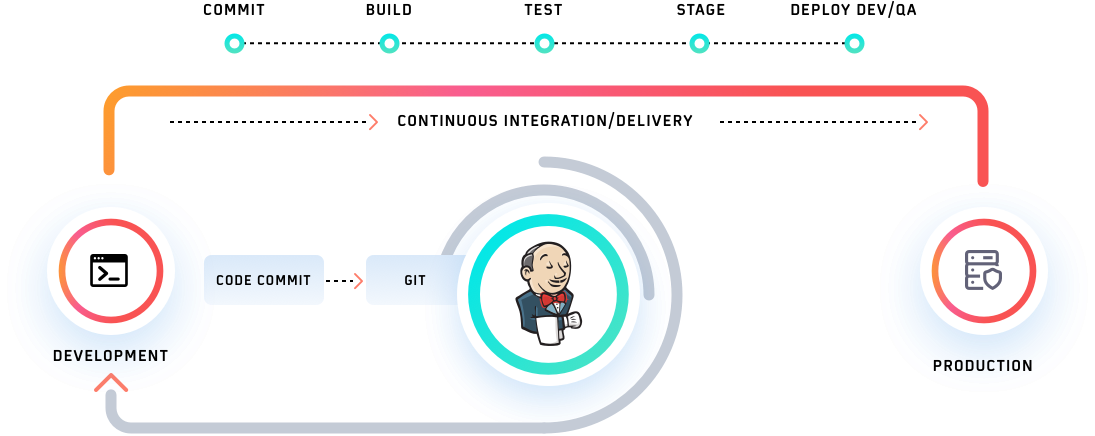
\includegraphics[width=\textwidth]{jenkins_pipeline.png}
            \caption{Pipeline Concept}
            \label{fig:my_label}
        \end{figure}
    }
    \only<2>{
        \begin{itemize}
            \item Jenkins Pipeline is a suite of plugins which supports implementing and integrating continuous delivery pipelines into Jenkins.
            \item The definition of a Jenkins Pipeline is written into a text file (called a \textbf{Jenkinsfile}) which in turn can be committed to a project’s source control repository.
            \item A Jenkinsfile can be written using two types of syntax - \textbf{Declarative} and \textbf{Scripted}. (\textbf{Declarative} is suggested). Both uses \colorbox{pink}{$groovy$} syntax. 
        \end{itemize}
    }
    \only<3>{
        \begin{itemize}
            \item Both \textbf{Declarative} and \textbf{Scripted} Pipeline are Domain Specific Language(\textbf{DSL}) to describe portions of your software delivery pipeline.
            \item A Pipeline can be created in one of the following ways:
            \begin{itemize}
                \item Through \textcolor{cyan}{Blue Ocean} (\textcolor{cyan}{Blue Ocean} rethinks the user experience of Jenkins)
                \item Through the classic UI
                \item In SCM(Create a Jenkinsfile) - \textbf{recommended}
            \end{itemize}
        \end{itemize}    
    }
    
\end{frame}

\begin{frame}[fragile]{PipeLine Script Example}

    \begin{lstlisting}[language=Java]
        pipeline{
            agent any
            stages{
                stage("Build"){
                    steps{
                        echo "Hello World"
                    }
                }
            }
        } \end{lstlisting}
    \begin{itemize}
        \item \textbf{Stage}
        \begin{itemize}
            \item A stage block defines a conceptually distinct subset of tasks performed through the entire Pipeline (e.g. "Build", "Test" and "Deploy" stages)
        \end{itemize}
        \item \textbf{Step}
            \begin{itemize}
                \item A single task. Fundamentally, a step tells Jenkins what to do at a particular point in time. 
            \end{itemize}
    \end{itemize}
\end{frame}

\begin{frame}{Configure PipeLine}
    \only<1>{
        \begin{figure}
            \centering
            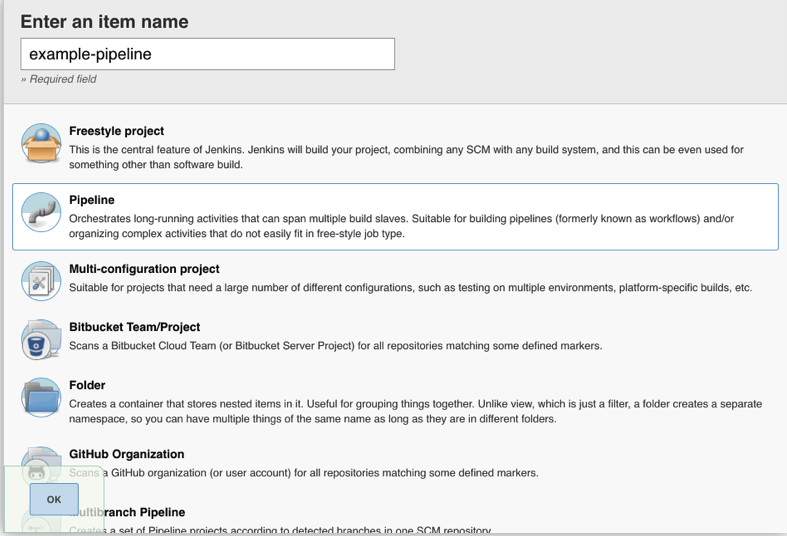
\includegraphics[width=\textwidth, height=6.5cm]{jenkins_configure_1.png}
            \caption{Choose Pipeline}
            \label{fig:Pipeline Configuration}
        \end{figure}
    }
    \only<2>{
        \renewcommand{\thefigure}{2}
        \begin{figure}
            \centering
            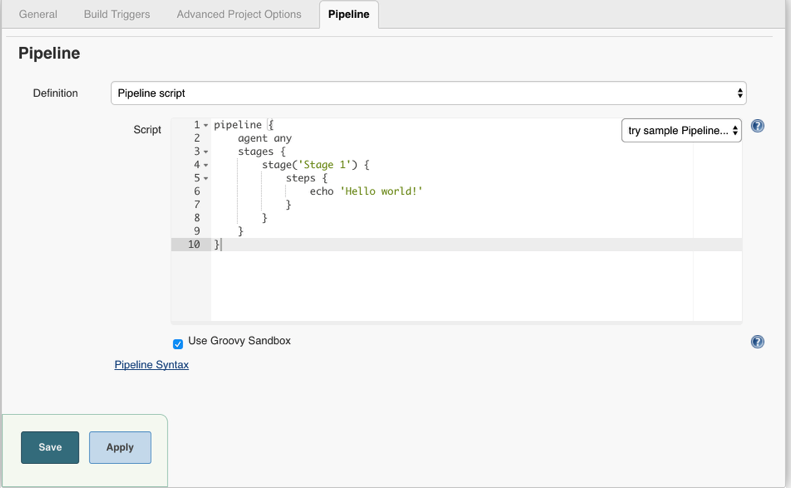
\includegraphics[width=\textwidth]{jenkins_configure_2.png}
            \caption{Pipeline through classic UI}
            \label{fig:Pipeline Configuration}
        \end{figure}
    }
    \only<3>{
        \renewcommand{\thefigure}{3}
        \begin{figure}
            \centering
            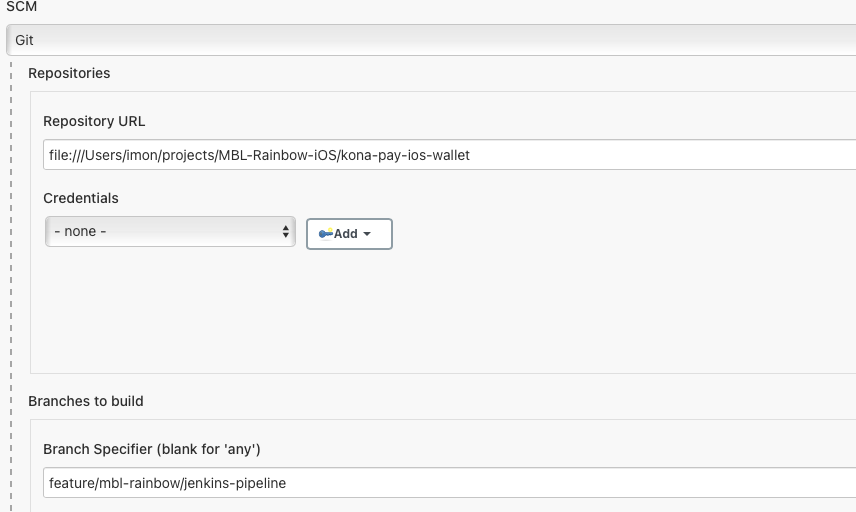
\includegraphics[width=\textwidth]{jenkins_configure_3.png}
            \caption{Set SCM info}
            \label{fig:Pipeline Configuration}
        \end{figure}
    }
    \only<4>{
        \renewcommand{\thefigure}{4}
        \begin{figure}
            \centering
            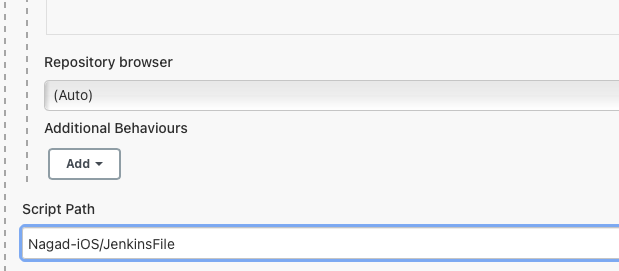
\includegraphics[width=\textwidth]{jenkins_configure_4.png}
            \caption{Point to Jenkinsfile location}
            \label{fig:Pipeline Configuration}
        \end{figure}
    }
\end{frame}

\begin{frame}{Pipeline Output}
    \only<1>{
        \renewcommand{\thefigure}{5}
        \begin{figure}
            \centering
            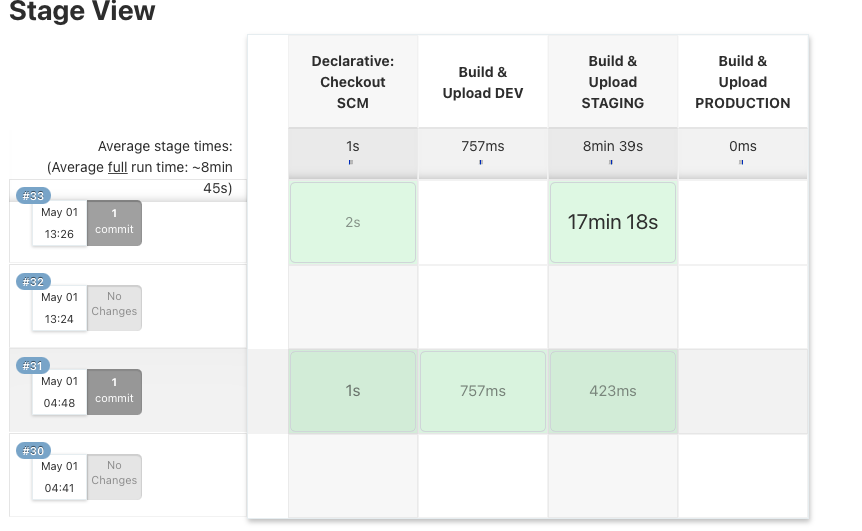
\includegraphics[width=\textwidth]{jenkins_output_classic.png}
            \caption{Pipeline Output in \textbf{Classic UI}}
            \label{fig:my_label}
        \end{figure}
    }
    
    \only<2>{
        \renewcommand{\thefigure}{6}
        \begin{figure}
            \centering
            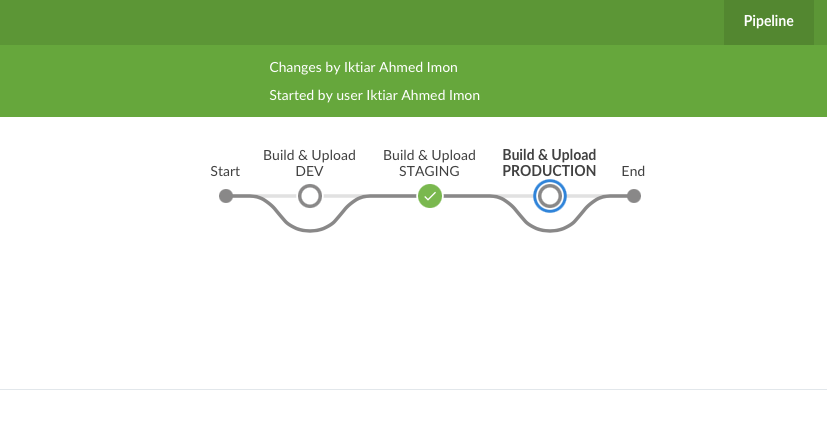
\includegraphics[width=\textwidth]{jenkins_output_blue_ocean.png}
            \caption{Pipeline Output in \textcolor{cyan}{Blue Ocean}}
            \label{fig:my_label}
        \end{figure}
    }

    
\end{frame}

\begin{frame}{Q \& A}
    \begin{figure}
        \centering
        
\includegraphics[width=\textwidth]{any_question.jpg}
        \label{fig:my_label}
    \end{figure}
\end{frame}

\begin{frame}[standout]
    Thank You All
\end{frame}

\end{document}

